\chapter{Coleta de Dados}
\label{cap:coleta-dados}

Para esta pesquisa, será utilizado uma base de dados com os nomes de todos os pacotes do \Gls{NPM} até jun/2017. Há nesta base de dados \textit{366,629} nomes de pacotes. A quantidade de amostras para o estudo será de \textit{385} pacotes, com base em um cálculo amostral\footnote{https://pt.surveymonkey.com/mp/sample-size-calculator/} com 95\% de confiança e 5\% de margem de erro. Dos \textit{366K} de pacotes, a amostra de \textit{385} será recuperada sorteando um número no intervalo \textit{0-366,629}. Do pacote sorteado será recuperado o seu \textit{package.json} e verificado se o pacote cumpre quatro requisitos: possuir mais de 1 dependente --  se não houver dependentes, não há possibilidades do pacote sofrer \textit{breaking changes}; possuir pelo menos a última \textit{release} com \textit{script} de teste não vazio e diferente do \textit{script} padrão de teste do \gls{NPM}: \textit{Error: no test specified}; possuir a \textit{url} do repositório do pacote; e o repositório do pacote precisa existir -- será esperado de uma requisição \Gls{HTTP} para o repositório o código \textit{200} indicando sua existência. A Figura \ref{fig:package_json} exemplifica as informações pertinentes no \textit{package.json} do pacote \textit{raven@0.1.0}\footnote{http://registry.npmjs.org/raven}.

\begin{figure}
    \centering
    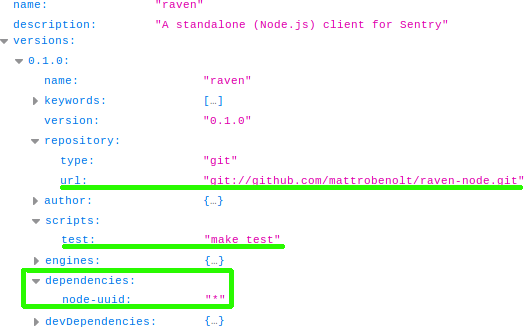
\includegraphics[scale=0.7]{figuras/package_json.png}
    \caption{Informações que serão recuperadas do \textit{package.json} para validar um pacote}
    \label{fig:package_json}
\end{figure}{}